\documentclass[12pt]{exam}
\usepackage[utf8]{inputenc}		% Caracteres latinos
\usepackage[spanish]{babel}		% Idioma español
\usepackage{geometry}			% Organizar el documento
\usepackage{graphicx}			% Incluir gráficos
\usepackage{makecell}			% Para personalizar las celdas de una tabla
\usepackage[nohdr]{mathexam}	% Añadimos el paquete mathexam (sin header)
\usepackage{amsmath}
\usepackage{amsfonts}
\usepackage{amssymb}
\usepackage{mathtools}
\usepackage{tikz}
\usepackage{pgfplots}
\pgfplotsset{compat=1.10}
\usepgfplotslibrary{fillbetween}
%\usetikzlibrary{positioning}    % yo
\usepgfplotslibrary{polar}
\usepackage[shortlabels]{enumitem}
\renewcommand{\baselinestretch}{1.5}
\usepackage{mathtools}
\usepackage{bm}
\usepackage{esvect}
\usepackage[fleqn]{mathtools}
\usepackage{relsize}
\usepackage{multirow}
\usepackage{multicol}
\usepackage[document]{ragged2e}
\usepackage{textpos}
\usepackage{tcolorbox}
\usepackage{hyperref}
%% \usepackage{wrapfig} % wrapfigure
%% \usepackage{float}
%% \usepackage{graphicx}
\usepackage{here} % [H]
\spanishdecimal{.}


\geometry{
  a4paper,                    % Tamaño del documento
  hmargin = {1.7cm, 1.7cm}, 	% Margen horizontal izquierdo, derecho
  vmargin = {1cm, 1cm},	    % Margen vertical superior, inferior
  headsep = 4mm,				% Separación entre el encabezado y el texto
  head = .2cm,				% Tamaño del encabezado
  % marginparsep = 5mm, 		% Seperación entre las notas y el texto
  % marginpar = 1.5cm,		% Tamaño de las notas
  includeall,                 % incluye el encabezado, footer y notas dentro del tamaño del documento
  nomarginpar,	            % Elimina las notas
  foot = 1cm,                 % Tamaño del footer
  twoside,                	% Habilita el modo de impresión a doble cara
}

\selectlanguage{spanish}       
\spanishdecimal{.}


\newcommand{\iuni}{\pmb{\hat{\imath}}}
\newcommand{\juni}{\pmb{\hat{\jmath}}}
\newcommand{\kuni}{\pmb{\hat{k}}}
% DOCUMENTO
\begin{document}

\centering


\Large 
\textbf{Tarea A}\\
\large 
Unidad 1: Integral de Riemann. Integrales dobles.\\
Alumno: Zarco Romero José Antonio\\
Valor: 7 puntos\\
\normalsize
Fecha de entrega: 

Viernes 23/08/2024 durante la clase

\vskip10pt

\normalsize

\pointpoints{punto}{puntos}
\pointformat{\bfseries\boldmath(\thepoints)}
\vskip10pt

\begin{questions}

  % ------------------------------------------------------------------------------------------------------------------------------------------------------------------------------------------------------------------------------
  \question
  
  \begin{multicols}{2}

    Usa una suma de Riemann con $m=n=2$ para estimar el valor de $\mathlarger{\iint}_R\text{sen}(x+y)dA$, donde $R=[0,\pi]\times[0,\pi]$. Elige los puntos muestra como las esquinas inferiores izquierdas.

    El valor de la integral doble de $f(x, y) = \sin{(x+y)}$ sobre el rectángulo $R=[0, \pi] \times [0,\pi]$, utilizando una \textbf{doble suma de Riemann} con $m=n=2$, es:

    \begin{figure}[H]
      \centering
      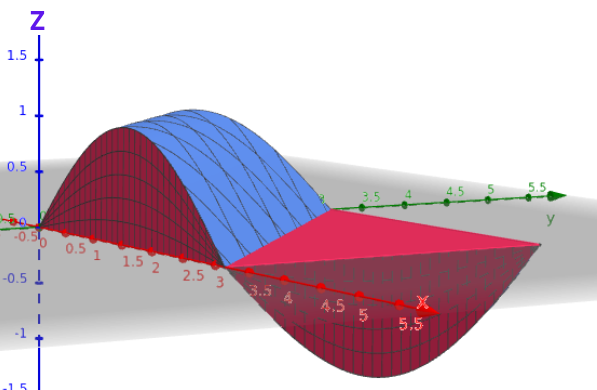
\includegraphics[width=0.45\textwidth]{{./img/t1a_1.png}}
      \label{fig:sen1}
      \caption{$\sin{(x+y)}$}
    \end{figure}
  \end{multicols}
  $$    \int \int _R f(x,y) dA  \approx \sum_{i=1}^{2}\sum_{j=1}^{2} f(x_{i-1},y_{j-1})\Delta A$$
  
  donde $x_{i-1}$ y $y_{j-1}$ son las \textit{esquinas inferiores izquierdas}. Además, $\Delta A = \Delta x \cdot \Delta y = \frac{\pi-0}{2} \cdot \frac{\pi-0}{2}=\frac{\pi}{2}\cdot\frac{\pi}{2} = \frac{\pi^2}{4}$

  \begin{figure}[H]
    \centering
    \begin{tikzpicture}
      % Dominio
      \draw[orange, very thick, fill=orange!6] (0,0) rectangle (4,4);
      \draw[orange, very thick] (2,0) -- (2,4);
      \draw[orange, very thick] (0,2) -- (4,2);

      % Ejes
      \draw[thick] (-1,0) -- (4.5,0) node[right] {$x$};
      \draw[thick] (0,-1) -- (0,4.5) node[above] {$y$};

      % Coordenadas
      \node at (0.6,0.4) {$(0, 0)$};
      \node at (0.6,2.4) {$\left(0, \frac{\pi}{2}\right)$};
      \node at (2.6,2.4) {$\left(\frac{\pi}{2}, \frac{\pi}{2}\right)$};
      \node at (2.6,0.4) {$\left(\frac{\pi}{2}, 0\right)$};

      % Regiones
      \node at (1,1) {$R_{11}$};
      \node at (1,3) {$R_{12}$};
      \node at (3,1) {$R_{21}$};
      \node at (3,3) {$R_{22}$};

      % Puntos
      \filldraw[black] (0,0) circle (2pt);
      \filldraw[black] (2,0) circle (2pt);
      \filldraw[black] (0,2) circle (2pt);
      \filldraw[black] (2,2) circle (2pt);
      
      % Escala
      \node at (-0.5,-0.5) {0};
      \node at (-0.5, 2) {$\frac{\pi}{2}$};
      \node at (-0.5,4) {$\pi$};
      \node at (2,-0.5) {$\frac{\pi}{2}$};
      \node at (4,-0.5) {$\pi$};
    \end{tikzpicture}
    \label{fig:rec1}
    \caption{Rectángulo $R$ de integración}
  \end{figure}

  Entonces,

  \begin{align*}
    \int \int _R \sin{(x+y)} dA
    &\approx \sum_{i=1}^{2}\sum_{j=1}^{2} \left[ f(x_{i-1},y_{j-1}) \cdot  \frac{\pi^2}{4} \right] \\
    &= \frac{\pi^2}{4} \left[ \sum_{i=1}^{2}\sum_{j=1}^{2} f(x_{i-1},y_{j-1}) \right] \\
    &= \frac{\pi^2}{4} \left[f(0,0)+f\left(0,\frac{\pi}{2}\right)+f\left(\frac{\pi}{2},0\right)+f\left(\frac{\pi}{2},\frac{\pi}{2}\right) \right] \\
    &= \frac{\pi^2}{4} \left[\sin{(0+0)}+\sin{\left(0+\frac{\pi}{2}\right)}+\sin{\left(\frac{\pi}{2}+0\right)}+\sin{\left(\frac{\pi}{2}+\frac{\pi}{2}\right)} \right] \\
    &= \frac{\pi^2}{4} \left[\sin{(0)}+\sin{\left(\frac{\pi}{2}\right)}+\sin{\left(\frac{\pi}{2}\right)}+\sin{(\pi)} \right] \\
    &= \frac{\pi^2}{4} \left(0+1+1+0 \right) \\
    &= \frac{\pi^2}{4} \cdot 2 \\
    &= \frac{\pi^2}{2} 
  \end{align*}
  Éste es el valor estimado de $f(x, y) = \sin{(x+y)}$

  % ------------------------------------------------------------------------------------------------------------------------------------------------------------------------------------------------------------------------------
  \question
  En la siguiente figura se muestra un mapa de curvas de nivel para la función $f(x,y)$. Usa la Regla del Punto Medio con $m=n=2$ para estimar el valor de $\mathlarger{\iint}_Rf(x,y)dA$ en la región $R=[0,4]\times[0,4]$. 
  \begin{figure}[H]
    \centering
    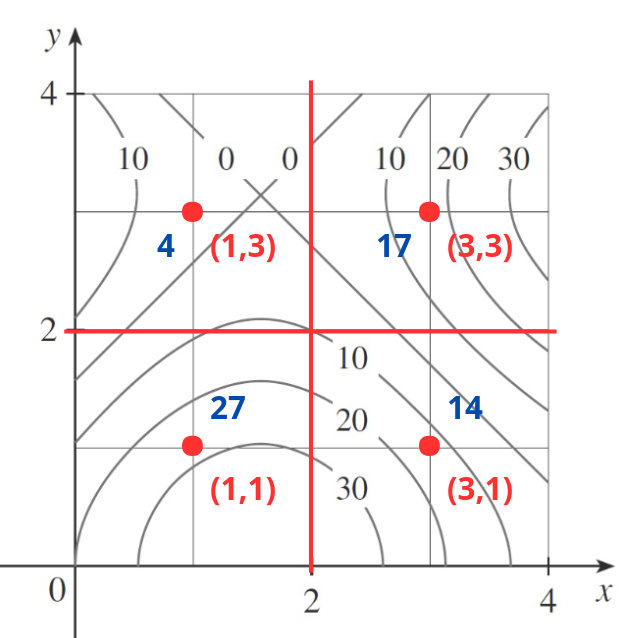
\includegraphics[width=0.4\textwidth]{{./img/t1a_2.png}}
    \label{fig:curvas}
    \caption{Curvas de nivel de $f(x,y)$}
  \end{figure}
  Utilizando la \textbf{Regla del punto medio para integrales dobles} donde
  $$ \iint\limits_{\underset{\textstyle R}{}} f(x,y)\, dA\approx \sum_{i=1}^{m} \sum_{j=1}^{n} f\left(\overline{x}_i, \overline{y}_j\right) \Delta A$$
  donde \( \overline{x}_i \) es el punto medio de \([x_{i-1}, x_i]\) y \( \overline{y}_j \) es el punto medio de \([y_{j-1}, y_j]\).

  El área de cada subrectángulo es $\Delta A=\Delta x \cdot\Delta y= \frac{4-0}{2}\cdot\frac{4-0}{2}=2\cdot 2=4$. Así que, al usar el \hyperref[fig:curvas]{mapa de contorno} para estimar el valor de $f$ en el centro de cada subrectángulo, obtenemos
  \begin{align*}
    \mathlarger{\iint}_Rf(x,y)dA
    &\approx \sum_{i=1}^{2} \sum_{j=1}^{2} \left[f\left(\overline{x}_i, \overline{y}_j\right) \cdot 4\right]\\
    &= 4 \left[\sum_{i=1}^{2} \sum_{j=1}^{2}f\left(\overline{x}_i, \overline{y}_j\right) \right]\\
    &= 4 \left[f(1,1)+f(1,3)+f(3,1)+f(3,3) \right]\\
    &= 4 \left(27+4+14+17\right) \\
    &= 4\cdot 62\\
    &= 248
  \end{align*}
  Por tanto, se tiene $\mathlarger{\iint}_Rf(x,y)dA \approx 248$

  % ------------------------------------------------------------------------------------------------------------------------------------------------------------------------------------------------------------------------------
  \question
  Calcula las siguientes integrales iteradas.
  \begin{enumerate}[a)]
  \item $\mathlarger{\int}_0^2\mathlarger{\int}_0^{1}(2x+y)^8\,dx\,dy$
    
    Si se considera a $y$ como una constante, se obtiene $ \int_{0}^{1} (2x+y)^8 dx $. Si hacemos que $u = 2x+y$, entonces
    $$ \frac{du}{dx}=2 \qquad \text{ así, } \qquad \frac{du}{2}=dx $$
    Además, los límites de integración quedan expresados como $u(0)=2(0)+y=y$ y $u(1)=2(1)+y=2+y$. De este modo,
    \begin{align*}
      \int_{0}^{1} (2x+y)^8 dx 
      &= \int_{y}^{2+y} u^8 \frac{du}{2}  \\
      &= \frac{1}{2} \int_{y}^{2+y} u^8 du \\
      &= \frac{1}{2} \left[ \frac{u^{8+1}}{8+1}\right]_y^{2+y} \\
      &= \frac{1}{2} \left[ \frac{u^9}{9}\right]_y^{2+y}  \\
      &= \frac{1}{2} \left\{ \left[ \frac{(2+y)^9}{9}\right] - \left[ \frac{y^9}{9}\right] \right\} \\
      &= \frac{1}{18} \left[ (2+y)^9 - y^9 \right] 
    \end{align*}
    Si ahora se integra la función respecto a $y$, se obtiene:
    \begin{align*}
      \int_{0}^{2}\int_{0}^{1} (2x+y)^8 dx dy
      &= \int_{0}^{2} \left[\int_{0}^{1} (2x+y)^8 dx \right] dy \\
      &= \int_{0}^{2} \left\{ \frac{1}{18} \left[ (2+y)^9 - y^9 \right] \right\} dy \\
      &= \frac{1}{18} \int_{0}^{2} \left[ (2+y)^9 - y^9 \right] dy \\
      &= \frac{1}{18} \left[ \int_0^2(2+y)^9dy - \int_0^2y^9dy \right]
    \end{align*}
    Resolviendo ambas integrales por separado, se tiene que:
    
    \begin{multicols}{2}
      \begin{itemize}[format=\textbf]
      \item $\int_0^2(2+y)^9dy$
        
        Si hacemos que $u=2+y$, entonces
        $$ \frac{du}{dy}=1 \qquad \text{ así, } \qquad du=dy $$
        Además, los límites de integración quedan expresados como $u(0)=2+(0)=2$ y $u(2)=2+(2)=4$. De este modo,
        \begin{align*}
          \int_0^2(2+y)^9dy
          &= \int_{2}^{4} u^9 du  \\
          &= \left[\frac{u^{9+1}}{9+1}\right]_{2}^{4}\\
          &= \left[\frac{u^{10}}{10}\right]_{2}^{4}\\
          &= \frac{4^{10}}{10} - \frac{2^{10}}{10} \\
          &= \frac{(2^2)^{10}-2^{10}}{10}\\
          &= \frac{2^{20}-2^{10}}{10}
        \end{align*}
      \item $\int_0^2y^9dy$
        \begin{align*}
          \int_0^2y^9dy
          &= \left[\frac{y^{9+1}}{9+1}\right]_0^2\\
          &= \left[\frac{y^{10}}{10}\right]_0^2\\
          &= \frac{(2)^{10}}{10} - \frac{(0)^{10}}{10} \\
          &= \frac{2^{10}}{10} - \frac{0}{10}\\
          &= \frac{2^{10}}{10} - 0\\
          &= \frac{2^{10}}{10}
        \end{align*}
      \end{itemize}
    \end{multicols}
    
    Luego, sustituyendo los valores de las integrales, se tiene que:
    \begin{align*}
      \frac{1}{18} \left[ \int_0^2(2+y)^9dy - \int_0^2y^9dy \right] 
      &= \frac{1}{18} \left[\left(\frac{2^{20}-2^{10}}{10}\right)-\left(\frac{2^{10}}{10}\right)\right]\\
      &= \frac{1}{18} \left(\frac{2^{20}-2^{10}-2^{10}}{10}\right) \\
      &= \frac{1}{18} \left[\frac{2^{20}-2(2^{10})}{10}\right] \\
      &= \frac{1}{18} \left(\frac{2^{20}-2^{11}}{10}\right) 
    \end{align*}
    \begin{align*}
      &= \frac{1}{18} \left[\frac{2(2^{19}-2^{10})}{10}\right] \\
      &= \frac{1}{18} \left(\frac{2^{19}-2^{10}}{5}\right) \\
      &= \frac{1}{18} \left[\frac{2(2^{18}-2^{9})}{5}\right] \\
      &= \frac{2}{18} \left(\frac{2^{18}-2^{9}}{5}\right) \\
      &= \frac{1}{9} \left(\frac{2^{18}-2^{9}}{5}\right) \\
      &= \frac{2^{18}-2^{9}}{45} \\
      &= \frac{2^{9}}{45} (2^9-1) \\
      &= \frac{261632}{45}
    \end{align*}
    $\therefore \mathlarger{\int}_0^2\mathlarger{\int}_0^{1}(2x+y)^8\,dx\,dy = \frac{2^{9}}{45} (2^9-1) \approx 5814.0444$
    \begin{figure}[H]
      \centering
      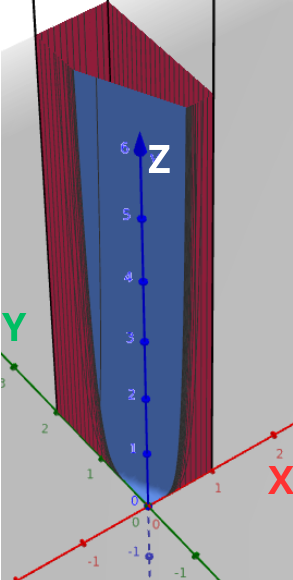
\includegraphics[scale=0.4]{{./img/t1a_3.png}}
      \label{fig:3a}
      \caption{$(2x+y)^8$}
    \end{figure}
    % --------------------------------------------------------------------------------
  \item $\mathlarger{\int}_{0}^{ln\,2}\mathlarger{\int}_{0}^{ln\,5}e^{2x-y}\,dx\,dy$

    Si se considera a $y$ como una constante, se obtiene $\mathlarger{\int}_{0}^{ln\,5}e^{2x-y}\,dx$. Si hacemos que $u=2x-y$, entonces
    $$\frac{du}{dx}=2 \qquad \text{ así, } \qquad \frac{du}{2}=dx$$
    Además los límites de integración quedan expresados como $u(\ln{\,5}) = 2(\ln{\,5})-y=2\ln{\,5}-y$ y $u(0)=2(0)-y=-y$. De este modo,
    \begin{align*}
      \mathlarger{\int}_{0}^{ln\,5}e^{2x-y}\,dx
      &= \mathlarger{\int}_{-y}^{2\ln{5}-y}e^{u}\, \frac{du}{2}  \\
      &= \frac{1}{2} \mathlarger{\int}_{-y}^{2\ln{5}-y}e^{u} \, du \\
      &= \frac{1}{2} \cdot e^u \Big| _{-y}^{2\ln{5}-y} \\
      &= \frac{1}{2} \left( e^{2\ln{5}-y}-e^{-y} \right) \\
      &= \frac{1}{2} \left( \frac{e^{2\ln{5}}}{e^y} - \frac{1}{e^y} \right) \\
      &= \frac{1}{2} \left( \frac{(e^{\ln{5}})^2}{e^y} - \frac{1}{e^y} \right) \\
      &= \frac{1}{2} \left( \frac{(5)^2}{e^y} - \frac{1}{e^y} \right) \\
      &= \frac{1}{2} \left( \frac{25}{e^y} - \frac{1}{e^y} \right) \\
      &= \frac{1}{2} \left( \frac{24}{e^y} \right) \\
      &= \frac{12}{e^y}
    \end{align*}
    Si ahora se integra la función respecto a $y$, se obtiene:
    \begin{align*}
      \mathlarger{\int}_{0}^{ln\,2}\mathlarger{\int}_{0}^{ln\,5}e^{2x-y}\,dx\,dy
      &= \mathlarger{\int}_{0}^{ln\,2}\left[\mathlarger{\int}_{0}^{ln\,5}e^{2x-y}\,dx\right]\,dy \\
      &= \mathlarger{\int}_{0}^{ln\,2}\left(\frac{12}{e^y}\right)\,dy \\
      &= 12\mathlarger{\int}_{0}^{ln\,2}e^{-y}\,dy
    \end{align*}
    Si hacemos $u=-y$, entonces  
    $$ \frac{du}{dy}=-1 \qquad \text{ así, } \qquad -du=dy $$
    Además, los límites de integración quedan expresados como $u(\ln{2})=-(\ln{2})=-\ln{2}$ y $u(0)=0$. De este modo,
    \begin{align*}
      12\mathlarger{\int}_{0}^{ln\,2}e^{-y}\,dy
      &= 12\mathlarger{\int}_{0}^{-\ln{2}}-e^{u}\,du \\
      &= -12\mathlarger{\int}_{0}^{-\ln{2}}e^{u}\,du \\
      &= 12\mathlarger{\int}_{-\ln{2}}^{0}e^{u}\,du 
    \end{align*}
    \begin{align*}
      &= 12 \cdot e^u \Big| _{-\ln{2}}^{0} \\
      &= 12 \left(e^{0}-e^{-\ln{2}}\right) \\
      &= 12\left(1-\frac{1}{e^{\ln{2}}}\right)\\
      &= 12\left(1-\frac{1}{2}\right)\\
      &= 12\left(\frac{1}{2}\right)\\
      &= 6
    \end{align*}
    $\therefore \mathlarger{\int}_{0}^{ln\,2}\mathlarger{\int}_{0}^{ln\,5}e^{2x-y}\,dx\,dy=6$
    \begin{figure}[H]
      \centering
      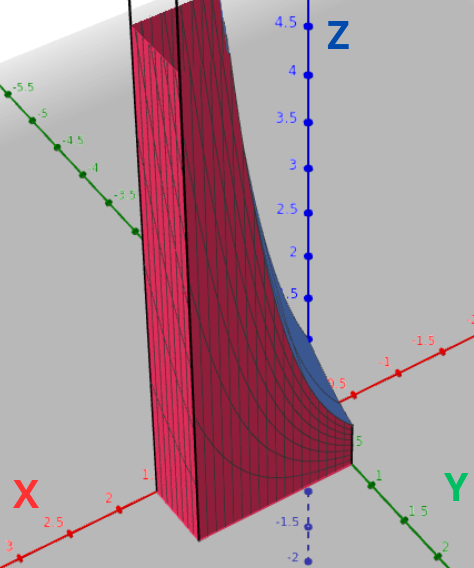
\includegraphics[scale=0.35]{{./img/t1a_3b.png}}
      \label{fig:3b}
      \caption{$e^{2x-y}$}
    \end{figure}
  \end{enumerate}
  % ------------------------------------------------------------------------------------------------------------------------------------------------------------------------------------------------------------------------------
  \question 
  Un cilindro recto no circular tiene su base $D$ en el plano $xy$ y está acotado superiormente por el paraboloide $z=x^2+y^2$. El volumen del sólido es $$V=\mathlarger{\int}_0^1\mathlarger{\int}_0^{y}(x^2+y^2)\,dx\,dy + \mathlarger{\int}_1^2\mathlarger{\int}_0^{2-y}(x^2+y^2)\,dx\,dy$$ 
  Dibuja la región D y expresa el volumen como una sola integral iterada con el orden de integración invertido. Finalmente evalúa la integral para encontrar el volumen. \\ \\
  

  De la ecuación del volumen del sólido podemos observar que cuando $y$ se encuentra entre 0 y 1, $x$ se mueve de 0 a $x=y$; asimismo cuando $y$ va de 1 a 2, $x$ se mueve de 0 a $x=2-y$. Así,
  
  \begin{figure}[H]
    \centering
    \begin{tikzpicture}
      \begin{axis}[
          legend pos=north east,
          axis lines = middle,
          xlabel = $x$,
          ylabel = $y$,
        ]
        
        \addplot[
          name path=f,
          thick,
          domain=-1:3, 
          color=red,
        ]
                {x};
                \addlegendentry{$y=x$}
                
                \addplot[
                  name path=g,
                  thick,
                  domain=-1:3, 
                  color=blue,
                ]
                        {2-x};
                        \addlegendentry{$y=2-x$}

                        \addplot[orange!35, opacity=0.4] fill between[of=f and g, soft clip={domain=0:1}];

                        
                        \draw [dashed, opacity=0.4] (axis cs:{1,0}) -- (axis cs:{1,1});
      \end{axis}
    \end{tikzpicture}
    \label{fig:4regiond}
    \caption{Región $D$}
  \end{figure}
  En la Figura \hyperref[fig:4regiond]{6} se ve que $D$ puede escribirse también como una región de tipo \textbf{I} por simplicidad:
  $$D=\{(x,y)~|~0\leq x\leq 1,~ x\leq y \leq 2-x \}$$
  Por tanto, otra expresión para $V$ es
  \begin{align*}
    V
    &=\mathlarger{\int}_0^1\mathlarger{\int}_{x}^{2-x}(x^2+y^2)\,dy\,dx \\
    &=\mathlarger{\int}_0^1\left[x^2y+\frac{y^3}{3}\right]_{x}^{2-x}\,dx\\
    &=\mathlarger{\int}_0^1\left\{\left[x^2(2-x)+\frac{(2-x)^3}{3}\right]-\left[x^2(x)+\frac{(x)^3}{3}\right]\right\}\,dx\\
    &=\mathlarger{\int}_0^1 \left[
      \left(2x^2-x^3+\frac{-x^3+6x^2-12x+8}{3}\right)
      -\left(x^3+\frac{x^3}{3}\right)
      \right]\,dx\\
    &=\mathlarger{\int}_0^1 
    \left(2x^2-x^3+\frac{-x^3+6x^2-12x+8}{3}
    -x^3-\frac{x^3}{3}\right)
    \right]\,dx\\
      &=\mathlarger{\int}_0^1 
      \left(
      2x^2-2x^3+\frac{-2x^3+6x^2-12x+8}{3}
      \right)
      \right]\,dx\\
        &= \mathlarger{\int}_0^1 
        \left(
        2x^2-2x^3-\frac{2}{3}x^3+2x^2-4x+\frac{8}{3}
        \right)
        \right]\,dx\\
          &= \mathlarger{\int}_0^1 
          \left(
          4x^2-\frac{8}{3}x^3-4x+\frac{8}{3}
          \right)
          \right]\,dx\\
            &=\left[
              \frac{4}{3}x^3-\frac{2}{3}x^4-2x^2+\frac{8}{3}x
              \right]_0^1\\
            &=\left[
              \frac{4}{3}(1)^3-\frac{2}{3}(1)^4-2(1)^2+\frac{8}{3}(1)
              \right]
            -\left[
              \frac{4}{3}(0)^3-\frac{2}{3}(0)^4-2(0)^2+\frac{8}{3}(0)
              \right]\\
            &=\left( \frac{4}{3}-\frac{2}{3}-2+\frac{8}{3}\right)-0
  \end{align*}
  \begin{align*}
    &= \frac{4}{3}
  \end{align*}
  $\therefore $ El volumen del sólido es de $\frac{4}{3}$ unidades cúbicas.
  %-------------------------------------------------------------------------------------------------------------------------------------------------------------------------------------------------------------------------
  \question
  Encuentra el volumen de los solidos con las siguientes características:
  \begin{enumerate}[a)]
  \item Acotado por la superficie $z=x\sqrt{x^2+y}$ y los planos $x=0$, $x=1$, $y=0$, $y=1$ y $z=0$.
    
    El volumen requerido se localiza debajo de la gráfica de la función $z=x\sqrt{x^2+y}$ y arriba de
    $$D=\{(x,y)~|~0\leq x\leq 1,~ 0\leq y\leq 1\}$$

    \begin{figure}[H]
      \centering
      \begin{tikzpicture}
        \begin{axis}[
            axis lines = middle,
            xlabel = $x$,
            ylabel = $y$,
            xmin=-0.5, xmax=1.5,
            ymin=-0.5, ymax=1.5,
            xtick={0,1},
            ytick={0,1},
            grid=major,
            legend pos=north east,
            clip=false
          ]
          
          % Sombra del cuadrado
          \addplot [
            draw=none,
            fill=orange,
            fill opacity=0.3,
          ]
          coordinates {(0,0) (1,0) (1,1) (0,1) (0,0)};
          
          % Dibujar el borde del cuadrado
          \addplot [
            thick,
            color=blue,
          ]
          coordinates {(0,0) (1,0) (1,1) (0,1) (0,0)};
          
          % Etiquetas de las líneas
          \node at (axis cs: 0.2,-0.2) [below] {$x=0$};
          \node at (axis cs: 1.2,-0.2) [below] {$x=1$};
          \node at (axis cs: -0.2,0.2) [left] {$y=0$};
          \node at (axis cs: -0.2,1.2) [left] {$y=1$};

        \end{axis}
      \end{tikzpicture}
      \label{fig:t1_5a}
      \caption{Región $D$}
    \end{figure}
    
    Por consiguiente,
    \begin{align*}
      V
      &= \mathlarger{\iint}_D \left(x\sqrt{x^2+y}\right)\,dA \\
      &= \mathlarger{\int}_0^1\mathlarger{\int}_0^1\left(x\sqrt{x^2+y}\right)\,dx\,dy\\
      &= \mathlarger{\int}_0^1\left[\mathlarger{\int}_0^1\left(x\sqrt{x^2+y}\right)\,dx\right]\,dy
    \end{align*}
    Si hacemos $u=x^2+y~\rightarrow ~ \frac{du}{dx}=2x$, así $\frac{du}{2}=x\,dx$. Además, $u(1)=1+y$ y $u(0)=y$. Entonces,
    \begin{align*}
      \mathlarger{\int}_0^1\left[\mathlarger{\int}_0^1\left(x\sqrt{x^2+y}\right)\,dx\right]\,dy
      &= \mathlarger{\int}_0^1\left[\mathlarger{\int}_{y}^{1+y}\left(\sqrt{u}\right)\,\frac{du}{2}\right]\,dy\\
      &= \mathlarger{\int}_0^1\left[\frac{1}{2}\mathlarger{\int}_{y}^{1+y}u^{\frac{1}{2}}\,du\right]\,dy\\
      &= \mathlarger{\int}_0^1\left\{\frac{1}{3}\left[(1+y)^{\frac{3}{2}}-(y)^{\frac{3}{2}}\right]\right\}\,dy\\
      &=\frac{1}{3}\mathlarger{\int}_0^1\left[(1+y)^{\frac{3}{2}}-y^{\frac{3}{2}}\right]\,dy
    \end{align*}
    \begin{align*}
      &= \frac{1}{3}\mathlarger{\int}_0^1(1+y)^{\frac{3}{2}}\, dy - \frac{1}{3}\mathlarger{\int}_0^1 y^{\frac{3}{2}}\,dy
    \end{align*}
    
    Resolviendo ambas integrales por separado, tenemos que:
    
    \begin{multicols}{2}
      \begin{itemize}[format=\textbf]
      \item $ \frac{1}{3}\mathlarger{\int}_0^1(1+y)^{\frac{3}{2}}\, dy$
        
        Si hacemos que $u=1+y$, entonces
        $$ \frac{du}{dy}=1 \qquad \text{ así, } \qquad du=dy $$
        Además, los límites de integración quedan expresados como $u(0)=1$ y $u(1)=2$. De este modo,
        \begin{align*}
          \frac{1}{3}\mathlarger{\int}_0^1(1+y)^{\frac{3}{2}}\, dy
          &= \frac{1}{3}\mathlarger{\int}_1^2 u^{\frac{3}{2}}\, du \\
          &= \frac{1}{3} \left[\frac{u^{\frac{5}{2}}}{\frac{5}{2}}\right]_1^2\\
          &= \frac{2}{15} \left[u^{\frac{5}{2}}\right]_1^2\\
          &= \frac{2}{15} (2^{\frac{5}{2}} - 1) \\
          &= \frac{2}{15} (4\sqrt{2} - 1) \\
          &= \frac{8\sqrt{2} - 2}{15}
        \end{align*}
      \item $\int_0^2y^9dy$
        \begin{align*}
          \frac{1}{3}\mathlarger{\int}_0^1 y^{\frac{3}{2}}\,dy
          &= \frac{1}{3} \left[\frac{y^{\frac{5}{2}}}{\frac{5}{2}}  \right]_0^1 \\
          &= \frac{2}{15}\left[y^{\frac{5}{2}} \right]_0^1 \\
          &= \frac{2}{15} (1-0) \\
          &=\frac{2}{15}
        \end{align*}
      \end{itemize}
    \end{multicols}

    Luego,

    \begin{align*}
      \frac{1}{3}\mathlarger{\int}_0^1(1+y)^{\frac{3}{2}}\, dy - \frac{1}{3}\mathlarger{\int}_0^1 y^{\frac{3}{2}}\,dy
      &= \frac{8\sqrt{2} - 2}{15} - \frac{2}{15} \\
      &= \frac{8\sqrt{2} - 4}{15}
    \end{align*}

    $\therefore$ El volumen del sólido es de $\frac{8\sqrt{2} - 4}{15} \approx 0.4875$ unidades cúbicas.
    
    %-------------------------------------------------------------------------------------------------------------
  \item Encerrado por los cilindros $z=x^2$, $y=x^2$ y los planos $z=0$ y $y=4$.
    Puesto que el segundo cilíndro parabólico corta al plano $xy$ (cuya ecuación es $z=0$) en la parábola $y=x^2$ y el segundo plano en la recta $y=4$. Se ve que el volumen $V$ está arriba de la región $D$ en el plano $xy$ acotado por la recta $y=4$ y la parábola $y=x^2$. (Véase la figura \hyperref[fig:5regionb]{8})
    \begin{figure}[H]
      \centering
      \begin{tikzpicture}
        \begin{axis}[
            legend pos=north east,
            axis lines = middle,
            xlabel = $x$,
            ylabel = $y$,
            domain=-3:3,
          ]
          
          \addplot[
            name path=f,
            thick,
            color=red,
          ]
                  {x^2};
                  \addlegendentry{$y=x^2$}
                  
                  \addplot[
                    name path=g,
                    thick, 
                    color=blue,
                  ]
                          {4};
                          \addlegendentry{$y=4$}

                          \addplot[orange!35, opacity=0.4] fill between[of=f and g, soft clip={domain=-2:2}];

                          
                          \draw [dashed, opacity=0.4] (axis cs:{2,0}) -- (axis cs:{2,4});
                          \draw [dashed, opacity=0.4] (axis cs:{-2,0}) -- (axis cs:{-2,4});
        \end{axis}
      \end{tikzpicture}
      \label{fig:5regionb}
      \caption{Región $D$}
    \end{figure}
    Así que el volumen requerido se localiza debajo de la gráfica de la función $z=x^2$ y arriba de
    $$D=\{(x,y)~|~-\sqrt{y} \leq x \leq \sqrt{y},~ 0\leq y\leq 4\}$$
    Por consiguiente,
    \begin{align*}
      V
      &= \mathlarger{\int}_0^4\mathlarger{\int}_{-\sqrt{y}}^{\sqrt{y}}x^2\,dx\,dy \\
      &= \mathlarger{\int}_0^4\left[\mathlarger{\int}_{-\sqrt{y}}^{\sqrt{y}}x^2\,dx\right]\,dy \\
      &= \mathlarger{\int}_0^4\left[\frac{x^{2+1}}{2+1}\right]_{-\sqrt{y}}^{\sqrt{y}}\,dy \\
      &= \mathlarger{\int}_0^4\left[\frac{x^3}{3}\right]_{-\sqrt{y}}^{\sqrt{y}}\,dy \\
      &= \mathlarger{\int}_0^4\left\{\left[\frac{(\sqrt{y})^3}{3}\right]-\left[\frac{(-\sqrt{y})^3}{3}\right]\right\}\,dy \\
      &= \mathlarger{\int}_0^4\left(\frac{y^{\frac{3}{2}}}{3}+\frac{y^{\frac{3}{2}}}{3}\right)\,dy\\
      &= \frac{2}{3}\mathlarger{\int}_0^4y^{\frac{3}{2}}\,dy
    \end{align*}
    \begin{align*}
      &= \frac{2}{3}\cdot \frac{y^{\frac{3}{2}+1}}{\frac{3}{2}+1} \Big|_0^4 \\
      &= \frac{2}{3}\cdot \frac{y^{\frac{3}{2}+1}}{\frac{5}{2}} \Big|_0^4 \\
      &=\frac{2}{3}\cdot \frac{2}{5}\cdot y^{\frac{5}{2}} \Big|_0^4 \\
      &=\frac{4}{15}\cdot \left[(4)^{\frac{5}{2}}-(0)^{\frac{5}{2}}\right] \\
      &=\frac{4}{15}\cdot \left(\sqrt{4^5}- 0) \\
      &=\frac{4}{15}\cdot \sqrt{1024} \\
      &=\frac{4}{15}\cdot 32 \\
      &=\frac{128}{15}
    \end{align*}
    \begin{figure}[H]
      \centering
      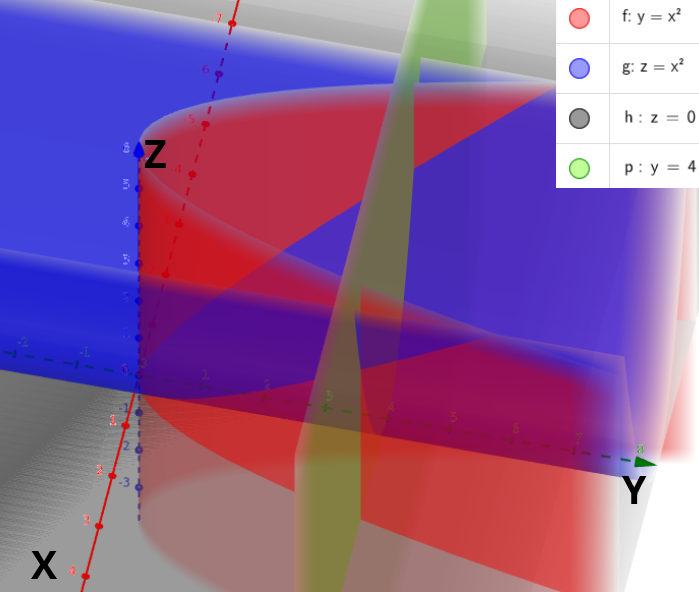
\includegraphics[width=0.5\textwidth]{{./img/t1a_5b.png}}
      \label{fig:5b}
      \caption{Sólido $5b)$}
    \end{figure}
    $\therefore$ El volúmen del sólido es de $\frac{128}{15} \approx 8.5333$ unidades cúbicas.
    
  \end{enumerate}

  \question
  Evalúa la integral invirtiendo el orden de integración.
  \begin{enumerate}[a)]
  \item $\mathlarger{\int}_0^1\mathlarger{\int}_{3y}^3 e^{x^2}\,dx\,dy$

    La región $D$ acotada por la recta $x=3y$ y $x=3$ con $y=0$ y $y=1$ se muestra en la figura \hyperref[fig:6regiona]{10}
    \begin{figure}[H]
      \centering
      \begin{tikzpicture}
        \begin{axis}[
            legend pos=north east,
            axis lines = middle,
            xlabel = $x$,
            ylabel = $y$,
            domain=0:3,
            ymin=0, ymax=2,
          ]
          
          % Plot the line y = 1/3 * x
          \addplot[
            name path=h,
            thick,
            color=red,
          ]
                  {1/3*x};
                  \node[color=red] at (axis cs: 1,0.7) {$y=\frac{1}{3}x$};
                  
                  % Plot the vertical line x = 3
                  \addplot[
                    name path=p,
                    thick, 
                    color=blue,
                  ]
                  coordinates {(3,-1) (3,2)};
                  \node[color=blue] at (axis cs: 2.7,1.5) {$x=3$};

                  % Shade the area between the curves
                  \addplot[orange!35, opacity=0.4] fill between[
                    of=h and p
                  ];

                  \draw [dashed, opacity=0.4] (axis cs:{0,1}) -- (axis cs:{3,1});

        \end{axis}
      \end{tikzpicture}
      \label{fig:6regiona}
      \caption{Región $D$}
    \end{figure}
    Si se hubiera expresado a $D$ como una región \textbf{tipo I}, entonces se abría obtenido:
    $$D=\left\{(x,y)~|~0 \leq x\leq 3,~ 0 \leq y\leq \frac{1}{3}x\right\}$$
    Con lo cual,
    \begin{align*}
      \iint\limits_{\underset{\textstyle D}{}} e^{x^2}\, dA
      &= \mathlarger{\int}_0^3\mathlarger{\int}_0^{\frac{1}{3}x} e^{x^2}\, dy\,dx \\
      &= \mathlarger{\int}_0^3\left[\mathlarger{\int}_0^{\frac{1}{3}x} e^{x^2}\, dy\right]\,dx \\
      &= \mathlarger{\int}_0^3\left[e^{x^2}y\right]_0^{\frac{1}{3}x} \,dx \\
      &= \mathlarger{\int}_0^3\frac{1}{3}xe^{x^2} \,dx 
    \end{align*}
    Si hacemos $u=x^2 ~ \rightarrow ~ \frac{du}{dx}=2x$, así $x\,dx = \frac{du}{2}$. Asímismo $u(3)=9$ y $u(0)=0$. Entonces,
    \begin{align*}
      \iint\limits_{\underset{\textstyle D}{}} e^{x^2}\, dA
      &= \mathlarger{\int}_0^3\frac{1}{3}xe^{x^2} \,dx  \\
      &= \frac{1}{6} \int_0^9 e^u du \\
      &= \frac{1}{6} \cdot e^u \Big|_0^9\\
      &= \frac{1}{6} \cdot e^9-1
    \end{align*}
    $\therefore$ Invirtiendo el orden de integración tenemos que $\mathlarger{\int}_0^3\mathlarger{\int}_0^{\frac{1}{3}x} e^{x^2}\, dy\,dx = \frac{e^9-1}{6}$
    
  \item $\mathlarger{\int}_0^1\mathlarger{\int}_{\text{arcsen}\,y}^{\pi/2}\text{cos}(x)\sqrt{1+\text{cos}^2x}\,dx\,dy$

    La región $D$ acotada por la función $x=\arcsen{(y)}$ y $x=\frac{\pi}{2}$ con $y=0$ y $y=1$ se muestra en la figura \hyperref[fig:6regionb]{11}
    \begin{figure}[H]
      \centering
      \begin{tikzpicture}
        \begin{axis}[
            axis lines = middle,
            xlabel = $x$,
            ylabel = $y$,
            domain=0:pi,
            samples=100,
            ymin=0, ymax=1.5,
            xmin=0, xmax=3.5,
            xtick={0, pi/2, pi},
            xticklabels={$0$, $\frac{\pi}{2}$, $\pi$},
            legend pos=north east
          ]
          
          % Plot the sine function y = sin(x)
          \addplot[
            name path=sine,
            thick,
            color=blue,
          ]
                  {sin(deg(x))};
                  \addlegendentry{$x=\arcsen{y}$}
                  
                  % Plot the vertical line x = pi/2
                  \addplot[
                    name path=line,
                    thick,
                    color=red,
                  ]
                  coordinates {(pi/2,-1.5) (pi/2,1.5)};
                  \addlegendentry{$x = \frac{\pi}{2}$}

                  % Plot the x-axis (y=0) as a path
                  \addplot[
                    name path=axis,
                    draw=none,
                    domain=0:pi/2,
                  ] 
                          {0};
                          
                          % Shade the area above y=0
                          \addplot [
                            thick,
                            color=orange,
                            fill=orange,
                            fill opacity=0.3,
                          ]
                          fill between[
                            of=sine and axis,
                            soft clip={domain=0:pi/2},
                          ];
                          \draw [dashed, opacity=0.4] (axis cs:{0,1}) -- (axis cs:{pi/2,1});

        \end{axis}
      \end{tikzpicture}
      \label{fig:6regionb}
      \caption{Región $D$}
    \end{figure}

    Si se hubiera expresado a $D$ como una región \textbf{tipo I}, entonces se abría obtenido:
    $$D=\left\{(x,y)~|~0 \leq x\leq \frac{\pi}{2},~ 0 \leq y\leq \sin{x} \right\}$$

    Con lo cual,
    \begin{align*}
      \iint\limits_{\underset{\textstyle D}{}} \text{cos}(x)\sqrt{1+\text{cos}^2x}\, dA
      &= \mathlarger{\int}_0^{\frac{\pi}{2}}\mathlarger{\int}_0^{\sin{x}} \text{cos}(x)\sqrt{1+\text{cos}^2x}\, dy\,dx \\
      &= \mathlarger{\int}_0^{\frac{\pi}{2}}\left[ \text{cos}(x)\sqrt{1+\text{cos}^2x}\cdot y\right]_0^{\sin{x}}\,dx \\
      &= \mathlarger{\int}_0^{\frac{\pi}{2}}\left( \text{sen}(x)\text{cos}(x)\sqrt{1+\text{cos}^2x}\right)\,dx 
    \end{align*}

    Si hacemos $u=\cos{x} ~\rightarrow~ \frac{du}{dx}=-\sin{x}$, así $-du=\sin{x\,dx}$. Además, $u(0)=1$ y $u(\frac{\pi}{2})=1$. De modo que,
    \begin{align*}
      \mathlarger{\int}_0^{\frac{\pi}{2}}\left( \text{sen}(x)\text{cos}(x)\sqrt{1+\text{cos}^2x}\right)\,dx
      &= 
      \mathlarger{\int}_1^0\left( -u\sqrt{1+u^2}\right)\,du \\
      &= \mathlarger{\int}_0^1\left( u\sqrt{1+u^2}\right)\,du \\
    \end{align*}
    Si hacemos $a=\sqrt{1+u^2}~\rightarrow ~ \frac{da}{du}=\frac{1}{2}(1+u^2)^{-\frac{1}{2}}\cdot 2u= \frac{u}{\sqrt{1+u^2}}$, así $u\,du = \sqrt{1+u^2}\, da=a\,da$. Además, $a(1)=\sqrt{2}$ y $a(0)=1$. Entonces, 
    \begin{align*}
      \mathlarger{\int}_0^1\left( u\sqrt{1+u^2}\right)\,du
      &= \mathlarger{\int}_1^{\sqrt{2}} (a\cdot a)\,da\\
      &= \mathlarger{\int}_1^{\sqrt{2}} a^2\,da\\
      &= \frac{a^3}{3}\Big|_1^{\sqrt{2}}\\
      &= \frac{2\sqrt{2}}{3}- \frac{1}{3}\\
      &= \frac{1}{3}\left(2\sqrt{2}-1\right)
    \end{align*}

    $\therefore$  Invirtiendo el orden de integración tenemos que $\mathlarger{\int}_0^{\frac{\pi}{2}}\mathlarger{\int}_0^{\sin{x}} \text{cos}(x)\sqrt{1+\text{cos}^2x}\, dy\,dx = \frac{1}{3}\left(2\sqrt{2}-1\right) \approx 0.6094$
  \end{enumerate}

  \question
  Encuentra el volumen del sólido $S$ como la diferencia entre dos volúmenes. $S$ es el sólido encerrado por los cilindros parabólicos $y=1-x^2$, $y=x^2-1$ y las planos $x+y+z=2$, $2x+2y-z+10=0$.

  \begin{itemize}
  \item Dado que el plano $x+y+z=2$ intersecta al plano $xy$ en $z=0$, se tiene que $x+y=2~\rightarrow ~y=2-x$ es la línea de intersección.
  \item Dado que el plano $2x+2y-z+10=0$ intersecta al plano $xy$ en $z=0$, se tiene que $2x+2y=-10~\rightarrow ~y=-5-x$ es la línea de intersección.
  \item Dado que los planos $x+y+z=2$ y $2x+2y-z+10=0$ se intersectan cuando los igualamos en $z$, se tiene que $2-x-y=2x+2y+10~\rightarrow ~ 3x+3y=-8 ~ \rightarrow ~ y = -x-\frac{8}{3}$ es la línea de intersección.
    \begin{itemize}
    \item Nótese que el plano $2x+2y-z+10=0$ se encuentra por encima del plano $x+y+z=2$ en el dominio
      $$D=\left\{(x,y)~|~-1\leq x\leq 1, ~ x^2-1\leq y \leq 1-x^2\right\}$$
    \end{itemize}
  \end{itemize}

  Así, se obtiene la región $D$ de integración del sólido $S$.
  
  \begin{figure}[H]
    \centering
    \begin{tikzpicture}
      \begin{axis}[
          axis lines = middle,
          xlabel = $x$,
          ylabel = $y$,
          domain=-3:3,
          samples=100,
          ymin=-6, ymax=3,
          xmin=-2.5, xmax=2.5,
          legend pos=south east,
          clip=false
        ]
        
        % Plot y = 1 - x^2
        \addplot[
          name path=curve1,
          thick,
          color=blue,
        ]
                {1 - x^2};
                \node[color=blue] at (axis cs: 2.7,-2) {$y = 1 - x^2$};
                
                % Plot y = x^2 - 1
                \addplot[
                  name path=curve2,
                  thick,
                  color=red,
                ]
                        {x^2 - 1};
                        \node[color=red] at (axis cs: 2.7,2) {$y = x^2 - 1$};

                        % Shade the area between y = 1 - x^2 and y = x^2 - 1
                        \addplot [
                          thick,
                          color=orange,
                          fill=orange,
                          fill opacity=0.3,
                        ]
                        fill between[
                          of=curve1 and curve2,
                          soft clip={domain=-1:1},
                        ];

                        % Plot y = 2 - x
                        \addplot[
                          thick,
                          color=green,
                        ]
                                {2 - x};
                                \node[color=green] at (axis cs: -0.5,4) {$y = 2 - x$};
                                
                                % Plot y = -5 - x
                                \addplot[
                                  thick,
                                  color=purple,
                                ]
                                        {-5 - x};
                                        \node[color=purple] at (axis cs: 1,-7.5) {$y = -5 - x$};

                                        % Plot y = -x - 8/3
                                        \addplot[
                                          thick,
                                          color=brown,
                                        ]
                                                {-x - 8/3};
                                                \node[color=brown] at (axis cs: 3.5,-4.4) {$y = -x - \frac{8}{3}$};

      \end{axis}
    \end{tikzpicture}
    \label{fig:t1a_7}
    \caption{Región $D$}
  \end{figure}

  Luego, el plano $2x+2y-z+10=0$ se puede escribir como $z=2x+2y+10$ y el plano $x+y+z=2$ puede escribirse como $z=-x-y+2$ también. De este modo, el volumen $V_s$ del sólido $S$ requerido se localiza debajo de la función  $z=2x+2y+10$ y arriba de la función $z=-x-y+2$ en la región $D$.
  
  \begin{figure}[H]
    \centering
    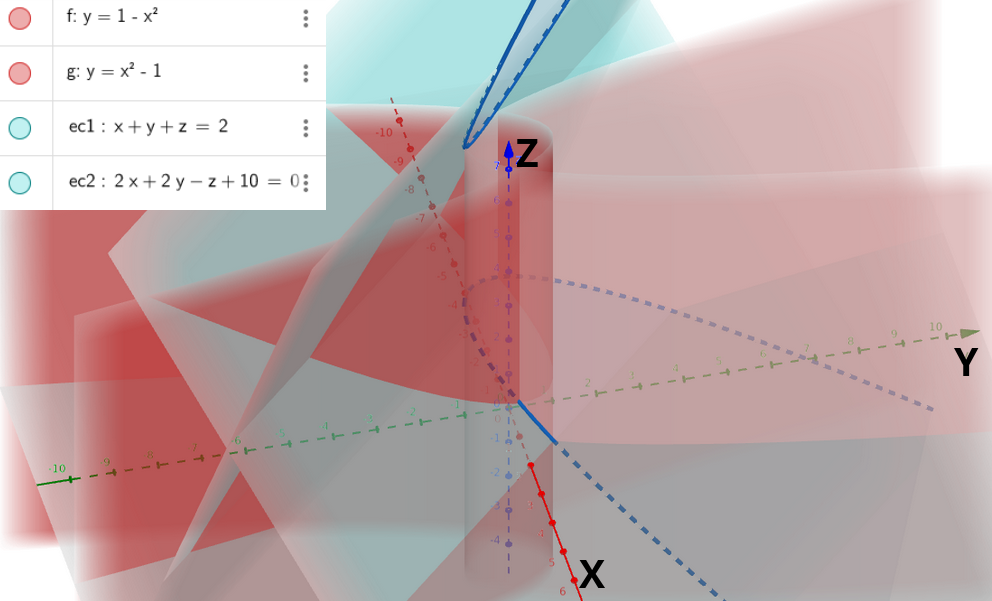
\includegraphics[scale=0.4]{{./img/t1a_7.png}}
    \label{fig:5b}
    \caption{Sólido $5b)$}
  \end{figure}

  Ahora, expresamos el volumen $V_s$ del sólido $S$ como la diferencia entre dos volúmenes
  \begin{align*}
    V_s
    &= \mathlarget{\int}_{-1}^1\mathlarget{\int}_{x^2-1}^{1-x^2} \left(2x+2y+10\right)\,dy\,dx
    - \mathlarget{\int}_{-1}^1\mathlarget{\int}_{x^2-1}^{1-x^2} \left(-x-y+2\right)\,dy\,dx\\
    &= \mathlarget{\int}_{-1}^1\mathlarget{\int}_{x^2-1}^{1-x^2} \left[(2x+2y+10)-(-x-y+2)\right]\,dy\,dx\\
    &= \mathlarget{\int}_{-1}^1\mathlarget{\int}_{x^2-1}^{1-x^2} (2x+2y+10+x+y-2)\,dy\,dx\\
    &= \mathlarget{\int}_{-1}^1\left[2xy+y^2+10y+xy+\frac{y^2}{2}-2y\right]_{x^2-1}^{1-x^2}\,dx\\
    &= \mathlarget{\int}_{-1}^1\left[3xy+8y+\frac{3y^2}{2}\right]_{x^2-1}^{1-x^2}\,dx\\
    &= \mathlarget{\int}_{-1}^1\left\{\left[3x(1-x^2)+8(1-x^2)+\frac{3(1-x^2)^2}{2}\right] - \left[3x(x^2-1)+8(x^2-1)+\frac{3(x^2-1)^2}{2}\right]\right\}\,dx\\
    &= \mathlarget{\int}_{-1}^1 [\left(3x-3x^3+8-8x^2+\frac{3}{2}-\frac{3}{2}x^2+\frac{3}{2}x^4\right)\\ &\qquad-\left(3x^3-3x+8x^2-8+\frac{3}{2}x^4-\frac{3}{2}x^2+\frac{3}{2}\right)] \,dx\\
    &= \mathlarget{\int}_{-1}^1 \left(-6x^3+6x-16x^2+16 \right)\,dx\\
    &= \left[-\frac{3}{2}x^4+3x^2-\frac{16}{3}x^3+16x\right]_{-1}^1\\
    &= \left[-\frac{3}{2}+3-\frac{16}{3}+16\right] - \left[-\frac{3}{2}+3+\frac{16}{3}-16\right]\\
    &= -\frac{32}{3}+32\\
    &=\frac{64}{3}
  \end{align*}

  $\therefore$ El volumen del sólido $S$ es $\frac{64}{3}\approx 21.3333$ unidades cúbicas.
  
\end{questions}
\vskip30pt
\RaggedRight

\newpage


\newgeometry {
  hmargin = {1.5cm, 1.5cm},
  vmargin = {5cm, 1cm},
  nohead,			% Elimina el encabezado
  nomarginpar,	% Elimina las notas
  includeall,
}% \savegeometry{geometria_1}

\pagestyle{foot}    % El estilo de ésta página sólo constará de pié de página
\runningfooter{}{}{Página \thepage\ de \numpages}

\end{document}
